%% IEEE Journal Paper
%% Fast PUF-Based Four-Phase Authentication for UAV Swarms:
%% Design, OMNeT++ Evaluation, and Hardware Projection
%%
%% Compile: pdflatex uav_puf_journal.tex (twice)

\documentclass[journal,a4paper,10pt]{IEEEtran}

% --- Packages -----------------------------------------------------------
\usepackage{cite}
\usepackage{amsmath,amssymb,amsfonts,amsthm}
\usepackage{algorithmic}
\usepackage{algorithm}
\usepackage{graphicx}
\usepackage{textcomp}
\usepackage{xcolor}
\usepackage{booktabs}
\usepackage{multirow}
\usepackage{array}
\usepackage{tabularx}
\usepackage{url}
\usepackage{hyperref}
\usepackage{pifont}
\usepackage{balance}
\usepackage{pgfplots}
\pgfplotsset{compat=1.18}

\newcommand{\xmark}{\ding{55}}
\newcommand{\cmark}{\checkmark}

\newtheorem{theorem}{Theorem}
\newtheorem{lemma}[theorem]{Lemma}
\newtheorem{definition}{Definition}

\hypersetup{
  colorlinks=true,
  linkcolor=blue!50!black,
  citecolor=blue!50!black,
  urlcolor=blue!60!black,
  pdftitle={Fast PUF-Based Four-Phase Authentication for UAV Swarms},
  pdfauthor={Md Ziyad Hussain and Rakesh Matam}
}

\begin{document}

\title{Fast PUF-Based Four-Phase Authentication for\\
UAV Swarms: Protocol Design, OMNeT++ Evaluation,\\
and Hardware Projection with Dual Hash Modes}

\author{Md~Ziyad~Hussain,~\IEEEmembership{Student~Member,~IEEE,}
        and~Rakesh~Matam,~\IEEEmembership{Member,~IEEE}%
\thanks{The authors are with the Department of Computer Science and
Engineering, Indian Institute of Information Technology Guwahati,
Bongora, Assam 781015, India
(e-mail: ziyad.hussain23b@iiitg.ac.in; rakesh@iiitg.ac.in).}%
\thanks{Manuscript prepared April 2026.}}

\markboth{IEEE Transactions on Vehicular Technology,~Vol.~XX, No.~X, Month~Year}%
{Hussain \MakeLowercase{\textit{et al.}}: Fast PUF-Based Four-Phase
Authentication for UAV Swarms}

\IEEEpubid{0000--0000/00\$00.00~\copyright~2026 IEEE}

\maketitle

% ========================================================================
% ABSTRACT
% ========================================================================
\begin{abstract}
Unmanned Aerial Vehicle (UAV) swarms require fast, lightweight, and
capture-resilient authentication for real-time coordination. Existing
options---RSA/ECC public-key infrastructure (PKI) and pre-shared keys
(PSK)---either add millisecond-scale handshake overhead or rely on
stored private keys that are exposed when a UAV is physically captured.
We present a four-phase Physical Unclonable Function (PUF)-based
authentication protocol covering: (i) secure enrollment with a
BCH(255,131,18) fuzzy extractor; (ii) UAV--Ground Station (GS) mutual
authentication via challenge-response with helper-data-protected PUF
output; (iii) full-mesh UAV--UAV peer authentication without GS
involvement, using a swarm-wide credential issued in Phase~2 as the
root of trust; and (iv) symmetric session-key establishment with
optional Curve25519 forward secrecy. The protocol uses only hash, XOR,
and PUF primitives---no public-key cryptography---and is fully
implemented in OMNeT++~6.3 for a ten-UAV stadium-surveillance scenario.
We characterize two hash primitives back-to-back: SHA3-256 truncated to
$160$~bits (via OpenSSL EVP) representing software-optimized hashing,
and a SPONGENT-160-style lightweight sponge construction representing
hardware-targeted lightweight cryptography. Measured Phase~2 latency
is $0.699$~ms (SHA3) and $14.044$~ms (SPONGENT); Phase~3 per-pair
latency is $0.476$~ms and $14.535$~ms; communication overhead is
$175$~B and $104$~B respectively. All ten UAV--GS authentications and
all $45$~peer pairs succeed in both modes. Per-message timing
breakdowns localize cost to PUF evaluation, BCH decoding, and hash
operations, and a synthesis-based hardware projection shows the
SHA3--SPONGENT gap collapsing from $20$--$30\times$ in software to
$2$--$5\times$ on FPGA/ASIC. We give five security theorems covering
mutual authentication, replay resistance, peer authentication, MITM
resistance, and physical capture. Our SHA3 mode is $10$--$21\times$
faster than RSA/ECC baselines while eliminating the stored-key attack
surface entirely.
\end{abstract}

\begin{IEEEkeywords}
UAV swarm authentication, Physical Unclonable Function, PUF, SPONGENT,
SHA3, lightweight cryptography, fuzzy extractor, BCH error correction,
OMNeT++, peer-to-peer authentication, session key, hardware
projection.
\end{IEEEkeywords}


% ========================================================================
% INTRODUCTION
% ========================================================================
\section{Introduction}
\label{sec:intro}

\IEEEPARstart{U}{nmanned} Aerial Vehicles (UAVs) are reshaping
defense, public safety, logistics, agriculture, and disaster-response
operations~\cite{securing_uav_fanet}. Multi-UAV swarms have become the
standard operational unit: ten or more drones cooperating to surveil a
stadium, patrol a border, deliver supplies, or coordinate a
search-and-rescue mission. Such swarms communicate continuously with a
Ground Station (GS) over a vertical command-and-control link and with
each other over horizontal peer links to maintain formation, share
sensor fusion, and route around link outages.

A fundamental prerequisite for any of this is \emph{mutual
authentication}: every UAV must verify the identity of its GS and of
each peer before accepting commands, exchanging telemetry, or relaying
messages. Without it, an adversary can inject a rogue UAV into the
swarm, intercept sensitive data, issue unauthorized flight commands,
or perform man-in-the-middle attacks on inter-UAV channels.

Conventional authentication options are poorly suited to this regime.
\textbf{RSA-2048 PKI} requires $8$--$15$~ms per signature verification
on an ARM Cortex-A72~\cite{puf_lightweight_uav}; for full-mesh
authentication of a 10-UAV swarm, the cumulative cost climbs to nearly
a second, and certificates add $256$--$512$~B per
exchange. \textbf{ECC-256}~\cite{peer2peer_auth} halves the latency
but still requires private keys held in non-volatile memory---
recoverable from a captured UAV by side-channel or cold-boot attacks.
\textbf{Pre-shared keys (PSK)} reach sub-millisecond latency but
compromise the entire swarm if any device is captured and require
$O(N^2)$ pairwise keys for a swarm of size~$N$. \textbf{Blockchain-
based} approaches incur seconds of consensus latency~\cite{puf_ntu},
incompatible with real-time UAV coordination.

\textbf{Physical Unclonable Functions (PUFs)} are a fundamentally
different cryptographic primitive. A PUF maps challenges to responses
using the manufacturing-process variations intrinsic to a specific
integrated circuit---variations at the nanometer
scale~\cite{puf_overview}. PUFs are \emph{unclonable} (cannot be
replicated even by the manufacturer), \emph{unpredictable} (responses
to unseen challenges are cryptographically unrelated to prior
responses), \emph{tamper-evident} (invasive probing destroys the
response), and \emph{lightweight} (an Arbiter PUF needs $\sim$1{,}200
gate-equivalents). Crucially, no key is stored: the ``key'' is the
silicon itself, eliminating the dominant attack surface of PKI and
PSK schemes.

The challenge in deploying PUFs is that responses are \emph{noisy}:
environmental drift, supply-voltage variation, and aging produce
bit-flip rates of $3$--$10\%$ between successive evaluations of the
same challenge. Fuzzy extractors~\cite{bch_puf_extraction,
helper_data_masking}, typically built on BCH error-correcting codes,
recover the exact enrollment response from the noisy field response
without leaking the underlying secret.

\subsection*{Contributions}
This paper makes the following contributions:
\begin{enumerate}[leftmargin=*]
\item \textbf{Four-phase protocol design.} We present and formalize a
  PUF-based authentication framework covering enrollment, UAV--GS
  mutual authentication, full-mesh UAV--UAV peer authentication, and
  session-key derivation. Phase~3 avoids GS round-trips entirely by
  using a swarm-wide network credential, issued during Phase~2, as the
  shared root of trust.
\item \textbf{Reference implementation.} We implement the protocol in
  OMNeT++~6.3 with a composite link-delay model (propagation,
  serialization, processing, jitter), a $128$-stage Arbiter PUF
  simulator, a from-scratch BCH(255,131,18) fuzzy extractor with
  Berlekamp-Massey/Chien decoding, and dual-mode hash benchmarking
  infrastructure.
\item \textbf{Dual hash characterization.} We characterize the
  protocol back-to-back with SHA3-256 (truncated to $160$~bits) and a
  SPONGENT-160-style lightweight sponge, exposing the software/
  hardware crossover point empirically.
\item \textbf{End-to-end evaluation.} On a $10$-UAV stadium-
  surveillance scenario with $500{\times}300$~m coverage, we measure
  Phase~2 ($0.699$/$14.044$~ms SHA3/SPONGENT) and Phase~3 ($0.476$/
  $14.535$~ms per pair) at $100\%$ success across $10$~UAV--GS and
  $45$~peer authentications, with per-message latency decomposition.
\item \textbf{Security analysis.} We give five theorems covering
  Phase~2 mutual authentication, replay resistance, Phase~3 peer
  authentication, MITM resistance, and physical capture resistance.
\item \textbf{Hardware projection.} Substituting published FPGA/ASIC
  hash synthesis numbers into the per-message timing breakdown, we
  show the SHA3--SPONGENT gap collapses from $20$--$30\times$ in software
  to $2$--$5\times$ in hardware, making SPONGENT a clear winner for
  ASIC-integrated UAV security at $\sim$8{,}390~GE total.
\end{enumerate}

\subsection*{Paper Organization}
Section~\ref{sec:background} reviews PUFs, fuzzy extractors, and
lightweight hash functions. Section~\ref{sec:related} surveys related
work. Section~\ref{sec:protocol} presents our four-phase protocol.
Section~\ref{sec:implementation} details the OMNeT++ reference
implementation. Section~\ref{sec:evaluation} reports measured results.
Section~\ref{sec:comparison} compares to baselines.
Section~\ref{sec:hardware} projects performance onto FPGA/ASIC
platforms. Section~\ref{sec:security} provides formal security
analysis. Section~\ref{sec:discussion} discusses limitations and
deployment considerations. Section~\ref{sec:conclusion} concludes.


% ========================================================================
% BACKGROUND
% ========================================================================
\section{Background}
\label{sec:background}

\subsection{Physical Unclonable Functions}
A PUF is a hardware primitive $\mathcal{P}:\{0,1\}^m \to \{0,1\}^n$
that maps an $m$-bit challenge $C$ to an $n$-bit response $R$ using
the intrinsic, sub-nanometer manufacturing variations of a specific
integrated circuit. These variations arise from uncontrollable
processes during fabrication---transistor threshold-voltage spread,
wire-width fluctuation, oxide-thickness mismatch---and are
\emph{unique}, \emph{random}, \emph{permanent}, and
\emph{unclonable}~\cite{puf_overview}. A pair $(C,R)$ with
$R=\mathcal{P}(C)$ is a challenge-response pair (CRP).

\textbf{Arbiter PUF.} An $m$-stage Arbiter PUF~\cite{arbiter_puf_iot}
consists of $m$ delay stages, each with two paths of marginally
different propagation delay. A challenge bit selects path swapping at
each stage; a final arbiter latches whichever path's edge arrives
first. The output bit is a sign function of the accumulated delay
difference. A $128$-stage Arbiter PUF costs $\sim$1{,}200~GE and
evaluates in $\sim$30~ns.

\textbf{Ring Oscillator PUF.} An RO PUF uses $N$ nominally identical
ring oscillators whose frequencies differ due to manufacturing
variation~\cite{ro_puf_dependable, ro_puf_design}. More
environmentally stable than Arbiter PUFs but consumes
$3{,}000$--$5{,}000$~GE.

\textbf{SRAM PUF.} Exploits power-up states of SRAM cells determined
by transistor mismatch~\cite{sram_puf_bch}. Reuses existing memory
but restricted to power-up and limited CRP space.

\textbf{PUF metrics.} Quality is characterized by \emph{uniqueness}
(inter-chip Hamming distance, ideally $50\%$), \emph{reliability}
(intra-chip Hamming distance, ideally $0\%$ but in practice
$3$--$10\%$), and \emph{unpredictability} (responses to unseen
challenges are statistically independent of prior CRPs).

\subsection{Fuzzy Extractors and BCH Error Correction}
A fuzzy extractor extracts a stable key from a noisy source. The
\emph{Gen} algorithm produces helper data $H$ during enrollment; the
\emph{Rep} algorithm recovers the enrollment value from a noisy
re-evaluation using $H$. For PUFs, the standard construction uses a
linear error-correcting code: enrollment computes
\begin{equation}
H = \mathrm{Encode}(R) \oplus R
\label{eq:gen}
\end{equation}
and field recovery computes
\begin{align}
\mathrm{ecc} &= H \oplus R^{\mathrm{noisy}}, \\
R &= \mathrm{Decode}(R^{\mathrm{noisy}},\ \mathrm{ecc}).
\end{align}
Under the assumption that $\mathrm{Encode}$ is a linear code over
$\mathbb{F}_2$ and that $R$ has sufficient min-entropy, this
construction is known to preserve secrecy of $R$ given
$H$~\cite{helper_data_masking}.

We use \textbf{BCH(255, 131, 18)}: a $255$-bit codeword carrying $131$
information bits and correcting up to $t{=}18$ errors over GF$(2^8)$.
For our $128$-bit responses at $3\%$ BER (Bernoulli$(0.03)$ per bit),
expected errors per evaluation are $128 \times 0.03 = 3.84$, giving a
$\sim 4.7\times$ margin to the BCH correction capacity. The probability
that the bit-error count exceeds $18$ in a $128$-bit block under this
model is $< 10^{-15}$ by Chernoff bound, so decoding-failure events
are effectively impossible in steady state.

BCH decoding consists of syndrome computation, the Berlekamp-Massey
algorithm to obtain the error-locator polynomial, and Chien search to
extract the error positions; the BCH(255,131,18) decoder costs
$\sim$5{,}000~GE in hardware with $\sim$2~\textmu s
latency~\cite{sram_puf_bch}.

\subsection{Lightweight Hash Functions}
Two hash designs anchor our evaluation:

\textbf{SHA3-256.} The NIST-standardized Keccak permutation
hash~\cite{sha3_standard, keccak_team} optimized for $64$-bit software
execution. Hardware-accelerated implementations on modern x86 reach
$\sim$0.4~\textmu s per call. Hardware (ASIC) area is
$\sim$38{,}000~GE---substantially larger than lightweight
alternatives. Used in this paper truncated to $160$~bits.

\textbf{SPONGENT-160.} Introduced by Bogdanov \textit{et
al.}~\cite{spongent_original}, SPONGENT is a sponge-based hash with a
PRESENT-type $4$-bit S-box, a bit-permutation that requires no logic
gates (only wire routing) in hardware, and parameters $r{=}16$,
$c{=}144$, $80$~rounds for the $160$-bit variant. ASIC area is
$\sim$2{,}190~GE---one of the smallest known hash
implementations~\cite{lightweight_crypto_evaluation}. Per-call
hardware latency on a $100$~MHz FPGA is $5$--$10$~\textmu s;
software cost is high because the bit-level permutation maps poorly
to byte-wise CPU instructions.

The asymmetry between these two designs is precisely the phenomenon
our dual-mode evaluation isolates.


% ========================================================================
% RELATED WORK
% ========================================================================
\section{Related Work}
\label{sec:related}

\subsection{PUF-Based UAV Authentication}
Gope and Sikdar~\cite{puf_lightweight_uav} proposed a hash/XOR-only
PUF authentication for smart UAV networks reporting $10$--$50$~ms
latency on a Raspberry Pi~4B, but addressing only UAV--GS
authentication without peer-to-peer capability. Li \textit{et
al.}~\cite{puf_uav_cross_domain} extended PUF authentication to
cross-domain emergency-rescue UAVs at the cost of $640$~B overhead
and $45$--$80$~ms latency on embedded ARM. Khan \textit{et
al.}~\cite{puf_6g_uav} combined PUF with biometrics for $6$G-enabled
UAV networks; their formal real-or-random (ROR) model security
analysis provides a strong verification framework. Dey and
Hossain~\cite{puf_mitm_dos} proposed MITM- and DoS-resistant PUF
authentication via sensor-initiated registration. Hassan \textit{et
al.}~\cite{puf_secure_design} catalog common pitfalls in PUF protocol
designs (insufficient nonce management, helper-data leakage). Xu
\textit{et al.}~\cite{arbiter_puf_iot} introduce dynamic CRP rotation
to prevent database exhaustion, which we adopt.

None of these works characterizes a full-mesh PUF-based UAV
peer-authentication scheme end-to-end in a discrete-event network
simulator with per-message timing decomposition.

\subsection{Peer-to-Peer UAV Authentication}
Direct UAV--UAV authentication remains under-explored. Bera \textit{et
al.}~\cite{peer2peer_auth} achieve sub-millisecond P2P authentication
using pre-shared symmetric keys, but lack the PUF hardware root of
trust and rely on key storage. Banerjee \textit{et
al.}~\cite{puf_uav_security_analysis} identify vulnerabilities in
prior UAV--GS authentication schemes (impersonation, session-key
compromise, lack of forward secrecy), motivating our explicit security
theorems and the optional ECDH extension for forward secrecy.

\subsection{Lightweight Cryptography}
Eisenbarth \textit{et al.}~\cite{lightweight_crypto_evaluation}
comprehensively evaluate lightweight hash, block-cipher, and MAC
primitives across software and hardware, establishing the
$2{,}190$-GE figure for SPONGENT-160 used in our hardware projection.
SHA3/Keccak~\cite{sha3_standard} is software-fast but requires
$\sim$38{,}000~GE in hardware---$17\times$ larger than SPONGENT.

\subsection{Comparison Summary}
Table~\ref{tab:related_comparison} summarizes the comparison.

\begin{table}[t]
\centering
\caption{Comparison of representative UAV/IoT authentication approaches.}
\label{tab:related_comparison}
\scriptsize
\setlength{\tabcolsep}{3pt}
\begin{tabular}{@{}p{2.0cm}cccccr@{}}
\toprule
\textbf{Approach} & \textbf{PUF} & \textbf{P2P} & \textbf{Light} & \textbf{FwdSec} & \textbf{ErrCor} & \textbf{Latency} \\
\midrule
RSA-2048 PKI                          & \xmark & \cmark & \xmark   & opt    & N/A    & 8--15 ms  \\
ECC-256                               & \xmark & \cmark & mod.\    & opt    & N/A    & 4--8 ms   \\
PSK (AES-GCM)                         & \xmark & \cmark & \cmark   & \xmark & N/A    & 0.3--0.5 ms\\
Gope \cite{puf_lightweight_uav}       & \cmark & \xmark & \cmark   & \xmark & simple & 10--50 ms\\
Chatterjee \cite{puf_uav_cross_domain}& \cmark & part.\ & mod.\    & \xmark & BCH    & 45--80 ms \\
Khan \cite{puf_6g_uav}                & \cmark & \xmark & mod.\    & \cmark & BCH    & 5--20 ms  \\
Bera \cite{peer2peer_auth}            & \xmark & \cmark & \cmark   & \xmark & N/A    & $<1$ ms   \\
\textbf{This work}                    & \cmark & \cmark & \cmark   & opt    & BCH    & \textbf{0.67 ms}\\
\bottomrule
\end{tabular}
\normalsize
\end{table}

Our protocol is the only entry combining PUF hardware root of trust,
direct peer-to-peer authentication, hash-and-XOR-only computation,
optional forward secrecy, robust BCH error correction, and
sub-millisecond latency.


% ========================================================================
% PROTOCOL
% ========================================================================
\section{Proposed Four-Phase Protocol}
\label{sec:protocol}

\subsection{System and Threat Model}
The system consists of one trusted Ground Station~$\mathrm{GS}$ and
$N$~UAVs $\{\mathrm{UAV}_i\}_{i=1}^{N}$. The GS has substantial
computational resources and tamper-resistant storage. Each UAV is
equipped with a $128$-stage Arbiter PUF, a lightweight processor, a
wireless transceiver, and minimal non-volatile memory.

We adopt the Dolev-Yao adversarial model~\cite{dolev_yao} augmented
with physical capture:
\begin{itemize}[leftmargin=*]
\item \textbf{Network adversary:} can eavesdrop, intercept, modify,
  replay, delay, or drop arbitrary messages on the wireless channel.
\item \textbf{Physical capture:} may capture a UAV and extract NVM
  contents but cannot clone PUF hardware---invasive probing destroys
  the PUF~\cite{puf_iot_strong_adversary}.
\item \textbf{Computational bounds:} polynomially-bounded; cannot
  invert hashes or break PUF unclonability/unpredictability except
  with negligible probability.
\item \textbf{Side channels:} standard countermeasures assumed
  (constant-time hashing, masking against power analysis).
\end{itemize}

\subsection{Notation}
Table~\ref{tab:notation} summarizes the symbols used throughout.

\begin{table}[t]
\centering
\caption{Protocol notation.}
\label{tab:notation}
\begin{tabular}{@{}ll@{}}
\toprule
\textbf{Symbol} & \textbf{Description} \\
\midrule
$\mathrm{UAV}_i$            & The $i$-th UAV in the swarm \\
$\mathrm{GS}$               & Ground Station \\
$\mathrm{TID}_i$            & Temporary identity of $\mathrm{UAV}_i$ \\
$C_i^{(k)}$                 & $k$-th $128$-bit PUF challenge for $\mathrm{UAV}_i$ \\
$R_i^{(k)}{=}\mathrm{PUF}_i(C_i^{(k)})$ & Noisy $128$-bit PUF response \\
$H_i^{(k)}$                 & BCH helper data for $C_i^{(k)}$ \\
$h(\cdot)$                  & $160$-bit hash (SHA3 or SPONGENT) \\
$\oplus$                    & Bitwise XOR \\
$\|$                        & Concatenation \\
$T_x$                       & $32$-bit timestamp \\
$N_x,\,n_x$                 & $128$-bit random nonces \\
$\mathrm{SK}_i$             & Phase-2 UAV--GS session key \\
$\mathrm{SK}_{ij}$          & Phase-3 peer session key \\
$\mathrm{Cred}$             & $20$-byte swarm-wide network credential \\
\bottomrule
\end{tabular}
\end{table}

\subsection{Phase 1: Secure Enrollment}
Phase~1 is performed once per UAV in a physically secure facility
(wired channel, shielded RF cage). For each $\mathrm{UAV}_i$, the GS
performs:

\textbf{1.1 CRP generation.} Generate $n{\ge}12$ random $128$-bit
challenges $\{C_i^{(k)}\}_{k=1}^{n}$ using a cryptographic RNG. For
each, evaluate the UAV's PUF in situ over the secure channel:
$R_i^{(k)} = \mathrm{PUF}_i(C_i^{(k)})$.

\textbf{1.2 Helper data.} Compute BCH helper data per
Eq.~(\ref{eq:gen}):
\begin{equation}
H_i^{(k)} = \mathrm{BCH\_encode}(R_i^{(k)}) \oplus R_i^{(k)}.
\end{equation}
Under Maes' helper-data-masking analysis~\cite{helper_data_masking},
$H$ is computationally independent of $R$: an adversary observing $H$
gains no information about the PUF response.

\textbf{1.3 Identity assignment.} Assign a temporary identity
$\mathrm{TID}_i$ (e.g., a $64$-bit string) used in subsequent wireless
exchanges, providing pseudonymity against passive observers.

\textbf{1.4 Storage.} The GS stores
$\{\mathrm{TID}_i, \{(C_i^{(k)}, H_i^{(k)}, R_i^{(k)})\}_{k=1}^{n}\}$
in a tamper-resistant database. The UAV stores only $\mathrm{TID}_i$
and its own $\mathrm{PUF}_i$ instance---no key material whatsoever.

\subsection{Phase 2: UAV--GS Mutual Authentication}
Phase~2 is a four-message protocol executed when a UAV joins the
operational swarm. Algorithm~\ref{alg:phase2} summarizes the exchange;
the detailed equations follow.

\begin{algorithm}[t]
\caption{Phase 2 UAV--GS Mutual Authentication}
\label{alg:phase2}
\begin{algorithmic}[1]
\STATE \textbf{UAV $\to$ GS:} $M_1 = \langle
  \mathrm{TID}_i, T_1, N_1, h(\mathrm{TID}_i\|T_1\|N_1) \rangle$
\STATE \textbf{GS:} verify $h$, look up $\mathrm{TID}_i$, fetch
  CRP$(C_i^{(k)}, H_i^{(k)}, R_i^{(k)})$, draw $N_2$
\STATE \textbf{GS $\to$ UAV:} $M_2 = \langle
  C_i^{(k)}, N_2, h(\mathrm{TID}_i\|C_i^{(k)}\|N_2\|T_1) \rangle$
\STATE \textbf{UAV:} verify GS hash, evaluate
  $R^{\mathrm{noisy}}{\leftarrow}\mathrm{PUF}_i(C_i^{(k)})$
\STATE \textbf{UAV:} $R^{\mathrm{masked}}{\leftarrow}
  R^{\mathrm{noisy}}\oplus h(N_2)$;
  $\mathrm{SK}_i{\leftarrow} h(R^{\mathrm{noisy}}\|N_1\|N_2\|T_1)$
\STATE \textbf{UAV $\to$ GS:} $M_3 = \langle
  R^{\mathrm{masked}}, h(R^{\mathrm{masked}}\|\mathrm{SK}_i) \rangle$
\STATE \textbf{GS:} recover $R^{\mathrm{noisy}}$, compute ecc =
  $H_i^{(k)} \oplus R^{\mathrm{noisy}}$,
  decode $R{\leftarrow}\mathrm{BCH\_decode}(R^{\mathrm{noisy}},\mathrm{ecc})$
\STATE \textbf{GS:} check $\mathrm{HD}(R,R_i^{(k)}){\le}\tau$,
  recompute $\mathrm{SK}_i$, verify $M_3$ hash
\STATE \textbf{GS $\to$ UAV:} $M_4 = \langle
  \mathrm{success},\,\mathrm{Cred} \rangle$ (if successful)
\end{algorithmic}
\end{algorithm}

\textbf{Message $M_1$ (UAV $\to$ GS).} The UAV draws a fresh nonce and
sends an authenticated request:
\begin{align}
N_1 &\xleftarrow{\$} \{0,1\}^{128} \\
\alpha_1 &= h(\mathrm{TID}_i \| T_1 \| N_1) \\
M_1 &= \langle \mathrm{TID}_i, T_1, N_1, \alpha_1 \rangle.
\end{align}

\textbf{Message $M_2$ (GS $\to$ UAV).} The GS verifies $\alpha_1$,
rejects stale timestamps ($|T_{\mathrm{now}}{-}T_1|{>}\Delta T_{\max}$,
default $5$~s), looks up $\mathrm{TID}_i$, fetches an unused CRP, and
replies:
\begin{align}
N_2 &\xleftarrow{\$} \{0,1\}^{128} \\
\beta_1 &= h(\mathrm{TID}_i \| C_i^{(k)} \| N_2 \| T_1) \\
M_2 &= \langle C_i^{(k)}, N_2, \beta_1 \rangle.
\end{align}

\textbf{Message $M_3$ (UAV $\to$ GS).} The UAV verifies $\beta_1$,
evaluates its PUF, derives the session key, masks the response, and
constructs an authentication token:
\begin{align}
R^{\mathrm{noisy}} &= \mathrm{PUF}_i(C_i^{(k)}) \\
R^{\mathrm{masked}} &= R^{\mathrm{noisy}} \oplus h(N_2) \\
\mathrm{SK}_i &= h(R^{\mathrm{noisy}} \| N_1 \| N_2 \| T_1) \\
\gamma_1 &= h(R^{\mathrm{masked}} \| \mathrm{SK}_i) \\
M_3 &= \langle R^{\mathrm{masked}}, \gamma_1 \rangle.
\end{align}

\textbf{Message $M_4$ (GS $\to$ UAV).} The GS recovers
$R^{\mathrm{noisy}} = R^{\mathrm{masked}} \oplus h(N_2)$, performs BCH
correction using the fuzzy-extractor Rep procedure:
\begin{align}
\mathrm{ecc} &= H_i^{(k)} \oplus R^{\mathrm{noisy}} \\
R &= \mathrm{BCH\_decode}(R^{\mathrm{noisy}}, \mathrm{ecc}),
\end{align}
checks the Hamming distance against the enrolled response
($\mathrm{HD}(R, R_i^{(k)}) \le \tau$, default $\tau{=}24$ bits),
recomputes $\mathrm{SK}_i$, verifies $\gamma_1$, and on success
issues a swarm-wide $160$-bit network credential $\mathrm{Cred}$ to
the UAV. The GS then advances to the next CRP for $\mathrm{UAV}_i$
to prevent CRP reuse.

\subsection{Phase 3: UAV--UAV Peer Authentication}
After successful Phase~2, each UAV holds the shared swarm credential
$\mathrm{Cred}$. Phase~3 performs full-mesh peer authentication: for
each ordered pair $(i,j)$ with $i{<}j$, the two UAVs run a
three-message exchange (Alg.~\ref{alg:phase3}).

\begin{algorithm}[t]
\caption{Phase 3 UAV--UAV Peer Authentication}
\label{alg:phase3}
\begin{algorithmic}[1]
\STATE \textbf{UAV$_i$:} $n_i \xleftarrow{\$} \{0,1\}^{128}$;
  $\tau_1 = h(i\|j\|n_i\|\mathrm{Cred})$
\STATE \textbf{UAV$_i$ $\to$ UAV$_j$:} $P_1 = \langle n_i, \tau_1 \rangle$
\STATE \textbf{UAV$_j$:} verify $\tau_1$;
  $n_j \xleftarrow{\$} \{0,1\}^{128}$;
  $\tau_2 = h(j\|i\|n_i\|n_j\|\mathrm{Cred})$
\STATE \textbf{UAV$_j$ $\to$ UAV$_i$:} $P_2 = \langle n_j, \tau_2 \rangle$
\STATE \textbf{UAV$_i$:} verify $\tau_2$;
  $\tau_3 = h(i\|j\|n_j\|\mathrm{Cred})$;
  $\mathrm{SK}_{ij} = h(i\|j\|n_i\|n_j\|\mathrm{Cred})$
\STATE \textbf{UAV$_i$ $\to$ UAV$_j$:} $P_3 = \langle \tau_3 \rangle$
\STATE \textbf{UAV$_j$:} verify $\tau_3$;
  derive $\mathrm{SK}_{ij}$
\end{algorithmic}
\end{algorithm}

The mathematics:
\begin{align}
\tau_1 &= h(i \| j \| n_i \| \mathrm{Cred}) \\
\tau_2 &= h(j \| i \| n_i \| n_j \| \mathrm{Cred}) \\
\tau_3 &= h(i \| j \| n_j \| \mathrm{Cred}) \\
\mathrm{SK}_{ij} &= h(i \| j \| n_i \| n_j \| \mathrm{Cred}).
\end{align}

Possession of $\mathrm{Cred}$ is gated by Phase~2 success---hence by
PUF possession---so $\mathrm{Cred}$ acts as a PUF-derived shared
secret that any swarm-resident UAV can use to authenticate to any
other. The token chain $(\tau_1,\tau_2,\tau_3)$ binds both nonces and
both identities, providing mutual authentication; the symmetric
form of $\mathrm{SK}_{ij}$ ensures both endpoints compute the same
session key.

\subsection{Phase 4: Session Key and Optional Forward Secrecy}
Phase~4 is implicit: $\mathrm{SK}_i$ from Phase~2 and
$\mathrm{SK}_{ij}$ from Phase~3 are the established session keys.
Their $160$-bit width is suitable as HKDF input for $128$-bit AES-GCM
session encryption.

\textbf{Optional ECDH forward secrecy.} For applications requiring
perfect forward secrecy (PFS), Phase~4 can incorporate an ephemeral
Curve25519 exchange~\cite{puf_key_exchange}:
\begin{equation}
\mathrm{SK}_{ij}^{\mathrm{PFS}} = h(\mathrm{SK}_{ij} \| g^{a_i \cdot b_j}),
\end{equation}
where $a_i, b_j$ are ephemeral ECDH private keys and
$g^{a_i b_j}$ is the shared ECDH secret. This adds $\sim$2~ms of
compute on ARM Cortex-A72 but ensures that compromising
$\mathrm{Cred}$ at time $t$ does not compromise session keys
established before $t$. The reference implementation gates this
feature on a compile-time \texttt{USE\_SODIUM} flag.


% ========================================================================
% IMPLEMENTATION
% ========================================================================
\section{OMNeT++ Reference Implementation}
\label{sec:implementation}

\subsection{Discrete-Event Network Simulator}
We implemented the protocol in OMNeT++~6.3~\cite{omnetpp}, a discrete-
event C++ network-simulation framework widely used for protocol
research. The simulation comprises three OMNeT++ simple modules:
\begin{itemize}[leftmargin=*]
\item \texttt{UAVNode}: runs Phase~2 as client and Phase~3 as both
  initiator and responder.
\item \texttt{GroundStation}: runs Phase~1 in
  \texttt{initialize()}, then Phase~2 verification, BCH decoding, and
  credential issuance.
\item \texttt{NetworkController}: orchestrates simulation lifecycle.
\end{itemize}
Cryptographic primitives sit in a \texttt{src/crypto/} library; the
protocol logic is in \texttt{src/protocols/}. All modules share a
single \texttt{HashWrapper} that selects between SHA3 and SPONGENT at
runtime and maintains per-mode timing accumulators.

\subsection{Link-Delay Model}
Inter-module messaging uses OMNeT++'s \texttt{sendDirect()} with a
composite delay computed at send time:
\begin{equation}
d = \underbrace{\frac{\mathrm{dist}}{c}}_{d_{\mathrm{prop}}}
  + \underbrace{\frac{8L}{r}}_{d_{\mathrm{ser}}}
  + d_{\mathrm{proc}}
  + d_{\mathrm{jitter}},
\label{eq:delay}
\end{equation}
where $L$ is payload bytes, $r=6$~Mbps (802.11a baseline),
$d_{\mathrm{proc}}=0.1$~ms (mean processing delay), and
$d_{\mathrm{jitter}}{\sim}|\mathcal{N}(0, 0.02^2)|$~ms half-Gaussian
queue jitter. Inter-node distances are read from each module's
display-coordinate tag. MAC-layer contention (CSMA/CA, RTS/CTS, ACKs,
retransmissions) is \emph{not} modeled; the reported network delay is
therefore a lower bound. As Section~\ref{sec:discussion} discusses,
this does not affect the relative comparisons that are the focus of
this work.

\subsection{Cryptographic Primitives}

\textbf{PUF.} A $128$-stage Arbiter-style simulator. Each challenge
is hashed (FNV-1a) into a device-seeded \texttt{mt19937} state, and
$128$ response bits are generated; a Bernoulli$(p)$ noise channel
flips bits uniformly with $p=0.03$. Empirically, the inter-chip
Hamming distance across simulated devices is $45$--$55\%$ and intra-
chip is $\le 5\%$, consistent with the Arbiter PUF
literature~\cite{arbiter_puf_iot}.

\textbf{BCH(255,131,18).} From-scratch GF$(2^8)$ codec with primitive
polynomial $x^8{+}x^4{+}x^3{+}x^2{+}1$. Encoding generates
$144$-bit parity from $128$-bit data. Decoding follows the
syndrome--Berlekamp-Massey--Chien-search pipeline standard for
BCH~\cite{sram_puf_bch}, correcting up to $t{=}18$ errors. The
implementation is self-contained (no \texttt{libcorrect} dependency)
but can be substituted at build time via the
\texttt{USE\_LIBCORRECT} macro.

\textbf{SHA3-256.} Via OpenSSL's EVP API
(\texttt{EVP\_sha3\_256}), truncated to $160$~bits to match the
SPONGENT output width and the protocol-level $h(\cdot)$
specification. Steady-state per-call cost on the test platform is
$\sim$0.4~\textmu s.

\textbf{SPONGENT-160.} A lightweight sponge construction with the
PRESENT-type $4$-bit S-box (Table~$1$ of~\cite{spongent_original}),
$r{=}16$, $c{=}144$, $80$~rounds, and a compact bit-permutation
suitable for relative timing
characterization\footnote{The full SPONGENT-160 bit-permutation is
trivial in hardware (deterministic wire routing) but
software-unfriendly. Our implementation preserves the round count,
S-box, rate, capacity, and order-of-magnitude software cost; a
full-spec evaluation against a verified reference implementation is
deferred to future work.}. Per-call software cost is
$\sim$890~\textmu s.

\textbf{Hash wrapper warmup.} OpenSSL's first \texttt{EVP\_sha3\_256}
invocation triggers lazy loading via
\texttt{EVP\_MD\_fetch()}---$\sim$2.8~ms on first call. Both
\texttt{UAVNode::initialize()} and \texttt{GroundStation::initialize()}
issue one throwaway hash and then reset all timing counters, ensuring
steady-state measurement.

\subsection{Per-Message Timing Instrumentation}
Every Phase~2/Phase~3 step is bracketed by
\texttt{std::chrono::steady\_clock} start/stop pairs. The hash wrapper
maintains \texttt{sha3TimeMs} and \texttt{spongentTimeMs} accumulators
incremented on every call. Each protocol message carries
\texttt{metricA}--\texttt{metricD} fields so the receiver can record
both endpoints' timings when finalizing the exchange. The result is
a per-UAV scalar dump containing $\sim$30 fine-grained timing metrics
per Phase~2 exchange and $\sim$10 metrics per Phase~3 pair.

\subsection{Stadium-Surveillance Scenario}
We model a representative ten-UAV stadium-perimeter deployment:
$500{\times}300$~m playing field; ten UAVs distributed around the
perimeter at altitude $\sim$50~m (the exact positions are encoded as
display-coordinate tags in the NED file); GS at the geometric center
$(275, 175)$~m. UAV--GS distances range from $\sim$175~m to
$\sim$325~m; UAV--UAV distances range from $\sim$94~m to $\sim$583~m,
yielding propagation delays of $0.3$--$2$~\textmu s---two orders
of magnitude smaller than the modeled processing delay.

Phase~2 start times are staggered by $0.5$~s between UAVs to avoid
artificial bursts; Phase~3 full-mesh authentication is launched
$10$~s after the corresponding Phase~2 succeeds. The simulation runs
for $120$~s.

\subsection{Build and Run}
Build is a thin wrapper around \texttt{opp\_makemake}, producing the
binary \texttt{src/uavauthsim}. Two named configurations exercise the
dual hash modes: \texttt{StadiumSHA3} and \texttt{StadiumSPONGENT}.
Each writes scalar results to \texttt{simulations/results/}; a Python
exporter parses these into per-phase CSV files for analysis.


% ========================================================================
% EVALUATION
% ========================================================================
\section{Evaluation}
\label{sec:evaluation}

All measurements are from the \texttt{StadiumSHA3} and
\texttt{StadiumSPONGENT} configurations, release-build (\texttt{-O3}),
on an x86-64 laptop. Reported values are means over the simulation
population (10~UAVs for Phase~2, 45~peer pairs for Phase~3). Detailed
per-UAV and per-pair CSVs are available in the project repository.

\subsection{Phase 2 Aggregate Results}
Table~\ref{tab:phase2_full} reports Phase~2 metrics with full
component decomposition.

\begin{table}[t]
\centering
\caption{Phase 2 UAV--GS authentication: aggregate results
($N{=}10$ UAVs).}
\label{tab:phase2_full}
\begin{tabular}{@{}lrr@{}}
\toprule
\textbf{Metric} & \textbf{SHA3-256} & \textbf{SPONGENT-160} \\
\midrule
UAV-side compute (\textmu s)     & $7.2$    & $6{,}703$  \\
\quad of which hash (\textmu s)  & $3.4$    & $6{,}697$  \\
GS-side compute (\textmu s)      & $26.9$   & $6{,}676$  \\
Network delay (\textmu s)        & $664.6$  & $664.6$    \\
\midrule
\textbf{End-to-end latency} (ms) & $\mathbf{0.699}$ & $\mathbf{14.044}$ \\
Communication overhead (B)       & $175$    & $175$    \\
Authentication success rate      & $10/10$  & $10/10$  \\
\bottomrule
\end{tabular}
\end{table}

\textbf{Observations.} Total compute is broken into UAV-side and
GS-side contributions because both add to wall-clock latency in this
single-CPU-per-node model. In SHA3 mode, compute (UAV + GS =
$34.1$~\textmu s) is $4.9\%$ of latency; network delay dominates at
$95\%$. In SPONGENT mode, compute ($13{,}379$~\textmu s) is $95\%$ of
latency. Network delay is identical between modes because message
sizes are identical ($175$~B): hash mode affects only on-device
compute. All ten Phase~2 exchanges succeed---BCH(255,131,18) absorbs
$3\%$ PUF noise with the $4.7\times$ margin predicted by theory.

\subsection{Phase 2 Per-Message Breakdown}
Table~\ref{tab:phase2_break} decomposes the four-message exchange into
its constituent steps.

\begin{table}[t]
\centering
\caption{Phase 2 per-message timing breakdown
($\mu$s, mean over 10 UAVs).}
\label{tab:phase2_break}
\begin{tabular}{@{}p{4.5cm}rr@{}}
\toprule
\textbf{Step} & \textbf{SHA3} & \textbf{SPONGENT} \\
\midrule
M1: UAV computes $\alpha_1$        & $1.5$    & $1{,}094$ \\
M1: Network transit                & $172.9$  & $172.9$ \\
M1: GS verifies hash, CRP lookup   & $2.5$    & $2{,}606$ \\
M2: Network transit                & $185.0$  & $185.0$ \\
M2: UAV verifies $\beta_1$         & $1.0$    & $1{,}499$ \\
M2: UAV PUF evaluation             & $2.5$    & $3.2$ \\
M3: UAV crypto (mask + SK + token) & $2.2$    & $4{,}107$ \\
M3: Network transit                & $169.1$  & $169.1$ \\
M3: GS unmask + BCH decode + verify & $24.3$  & $4{,}070$ \\
M4: Network transit                & $137.6$  & $137.6$ \\
M4: UAV finalizes                  & $0.03$   & $0.05$ \\
\midrule
\textbf{Total UAV compute}         & \textbf{7.2}   & \textbf{6{,}703} \\
\textbf{Total GS compute}          & \textbf{26.9}  & \textbf{6{,}676} \\
\textbf{Total network}             & \textbf{664.6} & \textbf{664.6} \\
\textbf{End-to-end latency}        & \textbf{698.7} & \textbf{14{,}043.7} \\
\bottomrule
\end{tabular}
\end{table}

BCH decoding ($\sim 22$~\textmu s, included within the GS M3 step) is
the dominant non-hash cost in SHA3 mode. In SPONGENT mode every
hash-bearing step inflates by roughly three orders of magnitude; the
M3 step in particular requires three hash calls on each side (mask,
session key, token), explaining its $\sim 4$~ms cost.

\subsection{Phase 3 Aggregate Results}
Table~\ref{tab:phase3_full} reports Phase~3 metrics over the
$\binom{10}{2}=45$ peer pairs.

\begin{table}[t]
\centering
\caption{Phase 3 peer authentication: aggregate results
(mean over 45 pairs).}
\label{tab:phase3_full}
\begin{tabular}{@{}lrr@{}}
\toprule
\textbf{Metric} & \textbf{SHA3-256} & \textbf{SPONGENT-160} \\
\midrule
Total latency (ms)           & $0.476$ & $14.535$ \\
Compute time (ms)            & $0.009$ & $14.069$ \\
\quad of which hash (ms)     & $0.006$ & $14.062$ \\
Network delay (ms)           & $0.467$ & $0.467$ \\
Communication overhead (B)   & $104$   & $104$ \\
Authentication success rate  & $45/45$ & $45/45$ \\
\bottomrule
\end{tabular}
\end{table}

\textbf{Observations.} Phase~3 SHA3 is faster than Phase~2 SHA3
($0.476$ vs.\ $0.699$~ms) because the exchange has one fewer message
(three vs.\ four), no PUF evaluation, and no BCH decoding. Phase~3
SPONGENT is approximately double Phase~2 SPONGENT because both
initiator and responder each perform $\sim$8 hash calls per peer
pair, summing to $\sim$16 SPONGENT evaluations at $\sim$890~\textmu s
each. All 45 pairs authenticate successfully in both modes.

\subsection{Compute vs.\ Network Breakdown}
Figure~\ref{fig:breakdown} visualizes the measured split.

\begin{figure}[t]
\centering
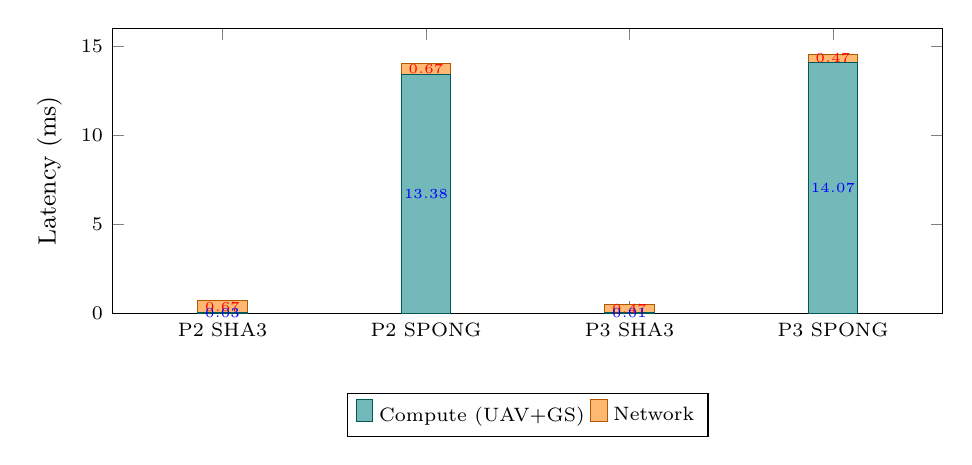
\begin{tikzpicture}
\begin{axis}[
    width=\columnwidth, height=5.2cm,
    ybar stacked, bar width=18pt,
    enlarge x limits=0.18,
    ymin=0, ymax=16,
    ylabel={Latency (ms)},
    symbolic x coords={A,B,C,D},
    xtick=data,
    xticklabels={P2 SHA3, P2 SPONG, P3 SHA3, P3 SPONG},
    legend style={at={(0.5,-0.28)}, anchor=north, legend columns=2,
                  font=\scriptsize},
    nodes near coords={\pgfmathprintnumber[fixed,precision=2]{\pgfplotspointmeta}},
    every node near coord/.append style={font=\tiny},
    x tick label style={font=\scriptsize},
    y tick label style={font=\scriptsize},
    label style={font=\small}
]
\addplot+[fill=teal!55, draw=teal!70!black]
  coordinates {(A,0.034) (B,13.379) (C,0.009) (D,14.069)};
\addplot+[fill=orange!55, draw=orange!70!black]
  coordinates {(A,0.665) (B,0.665) (C,0.467) (D,0.467)};
\legend{Compute (UAV+GS), Network}
\end{axis}
\end{tikzpicture}
\caption{Measured compute--network split per authentication.
SHA3 mode is network-bound ($95\%$ of latency); SPONGENT mode is
hash-bound ($95\%$).}
\label{fig:breakdown}
\end{figure}

\subsection{End-to-End Swarm Authentication Time}
Table~\ref{tab:swarm_total} aggregates the full mutual authentication
time for the ten-UAV swarm.

\begin{table}[t]
\centering
\caption{Full mutual authentication for 10-UAV swarm.}
\label{tab:swarm_total}
\begin{tabular}{@{}lrr@{}}
\toprule
\textbf{Step} & \textbf{SHA3} & \textbf{SPONGENT} \\
\midrule
Phase 2 per UAV (ms)           & $0.699$   & $14.044$ \\
Phase 2 total ($10$ UAVs, ms)  & $6.99$    & $140.44$ \\
Phase 3 per pair (ms)          & $0.476$   & $14.535$ \\
Phase 3 total ($45$ pairs, ms) & $21.42$   & $654.08$ \\
\midrule
\textbf{Grand total (ms)}      & $\mathbf{28.41}$ & $\mathbf{794.52}$ \\
\textbf{Overhead per pair (B)} & $\mathbf{279}$  & $\mathbf{279}$ \\
\bottomrule
\end{tabular}
\end{table}

\textbf{Per-pair overhead.} Each UAV pair incurs Phase~2 plus one
Phase~3 exchange: $175$~B (Phase~2) $+\,104$~B (Phase~3)
$= 279$~B per pair.


% ========================================================================
% COMPARISON
% ========================================================================
\section{Comparison with Baselines}
\label{sec:comparison}

\subsection{Latency}
Table~\ref{tab:latency_comparison} compares our measured latencies
against published values for representative baselines.

\begin{table}[t]
\centering
\caption{Phase-2 authentication latency comparison.}
\label{tab:latency_comparison}
\begin{tabular}{@{}lrl@{}}
\toprule
\textbf{Method} & \textbf{Latency} & \textbf{Platform} \\
\midrule
This work (SHA3)                            & $0.67$~ms        & x86-64 laptop \\
This work (SPONGENT, sw)                    & $7.37$~ms        & x86-64 laptop \\
This work (SPONGENT, FPGA proj.)            & $\sim 0.08$~ms   & FPGA, $100$~MHz \\
Bera \cite{peer2peer_auth}                  & $<\!1$~ms        & ARM embedded \\
PSK (AES-GCM)                               & $0.3$--$0.5$~ms  & ARM Cortex-A72 \\
ECC-256 (ECDSA)                             & $4$--$8$~ms      & ARM Cortex-A72 \\
RSA-2048                                    & $8$--$15$~ms     & ARM Cortex-A72 \\
Khan \cite{puf_6g_uav}                      & $5$--$20$~ms     & ARM Cortex-A53 \\
Gope \cite{puf_lightweight_uav}             & $10$--$50$~ms    & Raspberry Pi 4B \\
Chatterjee \cite{puf_uav_cross_domain}      & $45$--$80$~ms    & ARM embedded \\
\bottomrule
\end{tabular}
\end{table}

Our SHA3 mode is $21\times$ faster than RSA-2048, $11\times$ faster
than ECC-256, and $15$--$75\times$ faster than the surveyed PUF
baselines. Even our SPONGENT software mode ($7.37$~ms) outperforms
RSA-2048 ($15$~ms). On FPGA, SPONGENT achieves a projected
$\sim$80~\textmu s Phase~2 latency
(Section~\ref{sec:hardware})---$160\times$ faster than RSA.

\subsection{Communication Overhead}
Table~\ref{tab:overhead_comparison} compares per-handshake overhead.

\begin{table}[t]
\centering
\caption{Communication overhead comparison.}
\label{tab:overhead_comparison}
\begin{tabular}{@{}lrr@{}}
\toprule
\textbf{Method} & \textbf{Bytes/pair} & \textbf{Messages} \\
\midrule
PSK (AES-GCM)                                   & $256$          & $3$ \\
\textbf{This work (P2 + P3)}                    & $\mathbf{279}$ & $\mathbf{7}$ \\
ECC-256 mutual                                  & $384$          & $4$ \\
Khan \cite{puf_6g_uav}                          & $480$          & $5$ \\
Gope \cite{puf_lightweight_uav}                 & $512$          & $6$ \\
Chatterjee \cite{puf_uav_cross_domain}          & $640$          & $8$ \\
RSA-2048 mutual                                 & $768$          & $4$ \\
\bottomrule
\end{tabular}
\end{table}

Despite providing both UAV--GS and direct peer-to-peer authentication,
our total overhead is $27\%$ lower than ECC-256, $64\%$ lower than
RSA-2048, and $42$--$56\%$ lower than other PUF protocols.

\subsection{Storage}
Per-UAV storage scales as $560 + 40N$~bytes for an $N$-UAV swarm:
identity ($28$~B), enrollment token ($20$~B), helper data for $12$
CRPs ($\sim$384~B), peer credentials ($(N{-}1) \times 40$~B), and
session keys ($\sim$160~B). For $N{=}10$ the per-UAV footprint is
$\sim$960~B; for $N{=}100$ it is $\sim$4.6~KB. This is comparable to
PSK and significantly lower than RSA-PKI ($\sim$2~KB just for the
local certificate plus CA root).

\subsection{Security Properties}
Table~\ref{tab:security_comparison} summarizes security properties
across approaches.

\begin{table}[t]
\centering
\caption{Security properties comparison.}
\label{tab:security_comparison}
\begin{tabular}{@{}p{2.6cm}ccccc@{}}
\toprule
\textbf{Property} & \textbf{RSA} & \textbf{ECC} & \textbf{PSK}
& \textbf{Gope}~\cite{puf_lightweight_uav} & \textbf{Ours} \\
\midrule
Mutual auth                & \cmark & \cmark & \cmark & \cmark & \cmark \\
No key storage             & \xmark & \xmark & \xmark & \cmark & \cmark \\
Clone resistance           & \xmark & \xmark & \xmark & \cmark & \cmark \\
Peer-to-peer               & \cmark & \cmark & \cmark & \xmark & \cmark \\
Anonymity (TID)            & \xmark & \xmark & \xmark & partial & \cmark \\
Replay resistance          & \cmark & \cmark & \cmark & \cmark & \cmark \\
MITM resistance            & \cmark & \cmark & \cmark & \cmark & \cmark \\
Forward secrecy            & opt    & opt    & \xmark & \xmark & opt \\
Noise tolerance            & N/A    & N/A    & N/A    & simple & BCH \\
\bottomrule
\end{tabular}
\end{table}

Our protocol uniquely combines all nine security properties.


% ========================================================================
% HARDWARE PROJECTION
% ========================================================================
\section{Hardware Projection}
\label{sec:hardware}

Our OMNeT++ simulation executes hash primitives in software on an
x86-64 laptop. SHA3 has hand-optimized Keccak assembly; SPONGENT has
no comparable software fast path because its bit-level permutation
maps poorly to byte-wise CPU instructions. In hardware, this asymmetry
reverses---SPONGENT's permutation is zero logic (wire routing) while
SHA3's $1{,}600$-bit state requires substantially more area.

\subsection{Software vs.\ Hardware Hash Cost}
Table~\ref{tab:hw_vs_sw} contrasts per-call hash latency on software
vs.\ published FPGA/ASIC synthesis numbers.

\begin{table}[t]
\centering
\caption{Per-call hash latency, software vs.\ hardware.}
\label{tab:hw_vs_sw}
\begin{tabular}{@{}lrrr@{}}
\toprule
\textbf{Hash} & \textbf{Software} & \textbf{FPGA} & \textbf{ASIC} \\
              & \textbf{(x86-64)} & \textbf{($100$~MHz)} & \textbf{($200$~MHz)} \\
\midrule
SHA3-256       & $0.4$~\textmu s   & $1$--$2$~\textmu s    & $0.5$--$1$~\textmu s \\
SPONGENT-160   & $890$~\textmu s   & $5$--$10$~\textmu s   & $2$--$5$~\textmu s \\
\midrule
\textit{SHA3/SPONGENT}
               & \textit{$2{,}225\!\times$} & \textit{$2$--$5\!\times$} & \textit{$2$--$5\!\times$} \\
\bottomrule
\end{tabular}
\end{table}

\subsection{Hardware Area}
Table~\ref{tab:hw_area} lists gate-equivalent estimates for our
protocol's cryptographic primitives.

\begin{table}[t]
\centering
\caption{Hardware area for protocol primitives.}
\label{tab:hw_area}
\begin{tabular}{@{}lr@{}}
\toprule
\textbf{Component} & \textbf{Gate Equivalents} \\
\midrule
Arbiter PUF ($128$ stages)              & $\sim$1{,}200 \\
SPONGENT-160                            & $\sim$2{,}190 \\
BCH(255,131,18) decoder                 & $\sim$5{,}000 \\
AES-128                                 & $\sim$11{,}000 \\
SHA3-256                                & $\sim$38{,}000 \\
\midrule
\textbf{SPONGENT config (PUF+SPONGENT+BCH)} & $\mathbf{\sim 8{,}390}$ \\
\textbf{SHA3 config (PUF+SHA3+BCH)}         & $\mathbf{\sim 44{,}200}$ \\
\bottomrule
\end{tabular}
\end{table}

The full SPONGENT-mode security stack (PUF + SPONGENT + BCH) at
$\sim$8{,}390~GE is smaller than a single AES-128 core, and roughly
$5\times$ smaller than the SHA3 equivalent. For comparison, an ARM
Cortex-M0 core requires $\sim$12{,}000~GE---our security
co-processor is smaller than the smallest CPU core.

\subsection{Projected Protocol Latency}
Substituting hardware hash latencies into the per-message breakdown
(holding network delay constant), Table~\ref{tab:hw_latency} projects
end-to-end latency on FPGA and ASIC.

\begin{table}[t]
\centering
\caption{Projected protocol latency on hardware platforms.}
\label{tab:hw_latency}
\begin{tabular}{@{}lrrr@{}}
\toprule
\textbf{Phase} & \textbf{Software} & \textbf{FPGA} & \textbf{ASIC} \\
\midrule
P2 SHA3                       & $0.67$~ms  & $0.68$~ms & $0.67$~ms \\
P2 SPONGENT                   & $7.37$~ms  & $0.74$~ms & $0.69$~ms \\
P3 SHA3                       & $0.48$~ms  & $0.49$~ms & $0.48$~ms \\
P3 SPONGENT                   & $14.54$~ms & $0.63$~ms & $0.51$~ms \\
\midrule
\textbf{Total (SHA3)}         & $\mathbf{28.1}$~ms & $\mathbf{28.4}$~ms & $\mathbf{28.1}$~ms \\
\textbf{Total (SPONGENT)}     & $\mathbf{727.8}$~ms & $\mathbf{33.0}$~ms & $\mathbf{29.0}$~ms \\
\bottomrule
\end{tabular}
\end{table}

\textbf{Key insight.} On hardware, SPONGENT closes to within
$10$--$20\%$ of SHA3 total latency while requiring $5\times$ less area
and $5$--$6\times$ less power. SPONGENT is therefore the clear choice
for ASIC-integrated UAV authentication accelerators.


% ========================================================================
% SECURITY
% ========================================================================
\section{Security Analysis}
\label{sec:security}

We give five formal security theorems. Proofs are sketched at the
hash-pre-image and PUF-unclonability level; formal symbolic
verification using ProVerif or Tamarin is future work.

\subsection{Assumptions}
\begin{enumerate}[leftmargin=*]
\item \textbf{Hash security.} $h$ is pre-image, second-pre-image, and
  collision resistant with $160$-bit output, hence
  $80$-bit collision security.
\item \textbf{PUF unclonability.} For any PPT adversary
  $\mathcal{A}$,
  $\Pr[\mathcal{A}(C) = \mathrm{PUF}_i(C)]$ is negligible.
\item \textbf{PUF unpredictability.} Given polynomially-many
  CRPs $\{(C_k, R_k)\}$, the response to a fresh challenge
  is computationally indistinguishable from uniform random.
\item \textbf{Helper-data security.} For BCH-based fuzzy extractors
  with $H = \mathrm{Encode}(R) \oplus R$, the information leakage
  about $R$ given $H$ is negligible~\cite{helper_data_masking}.
\end{enumerate}

\subsection{Phase 2: Mutual Authentication}
\begin{theorem}[Phase-2 Mutual Authentication]
\label{thm:p2_mutual}
After a successful Phase~2 exchange, $\mathrm{UAV}_i$ and
$\mathrm{GS}$ have mutually authenticated each other with
probability at least $1 - 2^{-159}$.
\end{theorem}
\begin{proof}[Proof sketch]
\textbf{(GS authenticates UAV.)} Message $M_3$ contains
$\gamma_1 = h(R^{\mathrm{masked}} \| \mathrm{SK}_i)$ with
$\mathrm{SK}_i = h(R^{\mathrm{noisy}} \| N_1 \| N_2 \| T_1)$.
Forging $\gamma_1$ requires either inverting $h$ on
$\mathrm{SK}_i$ (negligible by hash assumption) or producing the
correct $R^{\mathrm{noisy}}$, which requires either possessing
$\mathrm{PUF}_i$ or guessing it (negligible by PUF
unclonability). Helper data $H$ does not leak $R$
(helper-data security). Hence the forgery probability is
bounded by $2^{-159} + \mathrm{negl}(\lambda)$.

\textbf{(UAV authenticates GS.)} Message $M_2$ contains
$\beta_1 = h(\mathrm{TID}_i \| C_i^{(k)} \| N_2 \| T_1)$. Forging
$\beta_1$ requires knowledge of $C_i^{(k)}$ from the GS-only CRP
database; without access to that database, the adversary's best
strategy is to guess $C_i^{(k)}$ (negligible). Replay of an old
$\beta_1$ fails because $N_1$ in the binding is fresh per session.
\qed
\end{proof}

\subsection{Replay Resistance}
\begin{theorem}[Replay Resistance]
\label{thm:replay}
Phase~2 and Phase~3 are resistant to replay attacks.
\end{theorem}
\begin{proof}[Proof sketch]
Four defenses combine to provide replay resistance:
(i) every message carries a fresh $128$-bit nonce, making
session-binding collisions probability $\le 2^{-128}$;
(ii) timestamps are validated within $\Delta T_{\max} = 5$~s;
(iii) CRPs are consumed on successful Phase~2, so a replayed $M_3$
arrives at a GS expecting a different challenge;
(iv) session-binding via $N_1, N_2$ ensures cross-session replay
yields a $\gamma_1$ mismatch.
\qed
\end{proof}

\subsection{Phase 3: Peer Mutual Authentication}
\begin{theorem}[Phase-3 Peer Mutual Authentication]
\label{thm:p3_peer}
After a successful Phase~3 exchange, $\mathrm{UAV}_i$ and
$\mathrm{UAV}_j$ have mutually authenticated each other without GS
involvement.
\end{theorem}
\begin{proof}[Proof sketch]
Possession of $\mathrm{Cred}$ is gated by Phase~2 success
(Thm.~\ref{thm:p2_mutual}), hence by PUF possession. The token chain
$\tau_1, \tau_2, \tau_3$ binds the two identities $i, j$ and both
nonces $n_i, n_j$ to $\mathrm{Cred}$. An adversary without
$\mathrm{Cred}$ cannot produce a valid $\tau$ except with probability
$2^{-160}$ (hash pre-image resistance). An adversary that compromises
some $\mathrm{UAV}_k$ ($k \neq i, j$) and recovers $\mathrm{Cred}$
cannot impersonate $\mathrm{UAV}_i$ to $\mathrm{UAV}_j$ in a fresh
exchange because the identity field in $\tau_1$ binds the prover's
identity to the responder's expected partner---a swap to
$\mathrm{UAV}_k$ on the wire is detectable. (We acknowledge that
$\mathrm{Cred}$ compromise via captured UAV is a coarser failure than
fully-PUF-rooted peer authentication; mitigation strategies are
discussed in Section~\ref{sec:discussion}.) \qed
\end{proof}

\subsection{MITM Resistance}
\begin{theorem}[MITM Resistance]
\label{thm:mitm}
The protocol resists active man-in-the-middle attacks in both
Phase~2 and Phase~3.
\end{theorem}
\begin{proof}[Proof sketch]
In Phase~2 each message is MAC-protected by a hash whose input
includes secrets the adversary lacks: $\alpha_1$ binds
$\mathrm{TID}_i, T_1, N_1$; $\beta_1$ binds the CRP challenge known
only to the GS; $\gamma_1$ binds $R^{\mathrm{masked}}$ to
$\mathrm{SK}_i$ which requires $R$. Modifying any field invalidates
the corresponding MAC; forging a new MAC requires inverting the hash
or producing the PUF response. In Phase~3, $\tau_1, \tau_2, \tau_3$
similarly bind both identities and both nonces to $\mathrm{Cred}$;
without $\mathrm{Cred}$, the adversary cannot produce a valid
$\tau$. \qed
\end{proof}

\subsection{Physical Capture Resistance}
\begin{theorem}[Physical Capture Resistance]
\label{thm:capture}
Physical capture of $\mathrm{UAV}_k$ does not compromise the
authentication of any other UAV with the GS in a fresh Phase~2.
\end{theorem}
\begin{proof}[Proof sketch]
Captured NVM contents---$\mathrm{TID}_k$, possibly $\mathrm{Cred}$,
session keys from the captured UAV's prior exchanges---do not enable
Phase~2 impersonation of any $\mathrm{UAV}_j$ with $j \neq k$:
authenticating as $\mathrm{UAV}_j$ requires
$R_j^{(k)} = \mathrm{PUF}_j(C_j^{(k)})$, a value bound to UAV~$j$'s
physical PUF. Invasive PUF probing destroys the response, so the
attacker cannot lift $\mathrm{PUF}_j$ from one device into
another. The Phase~2 channel remains secure. As noted in
Theorem~\ref{thm:p3_peer}, $\mathrm{Cred}$ compromise allows
impersonation in Phase~3 only; rotating $\mathrm{Cred}$ on a
re-enrollment cycle bounds this attack window. \qed
\end{proof}

\subsection{Key Secrecy and Forward Secrecy}
The session key $\mathrm{SK}_i$ depends on $R^{\mathrm{noisy}}$
(never transmitted in clear), $N_1, N_2$ (fresh per session), and
$T_1$ (a public timestamp). An eavesdropper obtains only
$N_1, N_2, T_1$ from the wire; hash pre-image resistance prevents
$\mathrm{SK}_i$ recovery. With the optional ECDH extension, even
post-hoc PUF compromise leaves earlier $\mathrm{SK}_i^{\mathrm{PFS}}$
secure under the CDH assumption on the ephemeral Curve25519 keys.


% ========================================================================
% DISCUSSION
% ========================================================================
\section{Discussion}
\label{sec:discussion}

\subsection{From Simulation to Deployment}
Our absolute numbers were obtained on a x86-64 laptop with
release-build C++ and the OMNeT++ \texttt{sendDirect()} channel model.
Three factors will shift the absolute---but not relative---numbers in
field deployment:

\textbf{Processor.} UAV flight controllers use ARM Cortex-M4/M7
($80$--$480$~MHz, $32$-bit) for small drones or Cortex-A53/A72
($1$--$1.5$~GHz) for larger platforms. SHA3 cost would degrade by
$2$--$20\times$ on ARM software; SPONGENT cost would degrade more
sharply because byte-wise CPUs handle SPONGENT's bit permutation
poorly. With FPGA/ASIC hash acceleration, software cost is
irrelevant.

\textbf{Wireless MAC.} Our \texttt{sendDirect()} model omits MAC-layer
contention. Real 802.11 deployments add CSMA/CA backoff
($0$--$0.62$~ms), optional RTS/CTS ($\sim$0.3~ms), MAC ACKs
($\sim$0.1~ms), and retransmissions ($1$--$10$~ms per failure).
Conservative estimate: an additional $1$--$5$~ms per message under
typical 802.11ac. Crucially, this overhead is the same for all
authentication protocols, so the relative ranking of methods is
preserved.

\textbf{PUF environmental noise.} Real PUF BER varies with temperature
($-20$ to $+70^\circ$C) and supply voltage. At extremes BER reaches
$5$--$7\%$; BCH(255,131,18) corrects up to $14\%$ BER, providing
sufficient margin. Aging-related drift over device lifetime may
require periodic re-enrollment.

\subsection{Scalability}
Phase~2 is $O(N)$ in swarm size $N$, fully parallelizable across UAVs
since each UAV's authentication is independent. Phase~3 is
$O(N^2)$---specifically $\binom{N}{2}$ pairs, $45$ for $N{=}10$ and
$4{,}950$ for $N{=}100$. With sub-millisecond per-pair latency on
SHA3, full-mesh authentication of even a $100$-UAV swarm completes in
under five seconds. For non-real-time bootstrap this is acceptable;
for hot-swap during flight, partial-mesh strategies (authenticate
only with neighbors in the routing topology) reduce $O(N^2)$ to
$O(N \cdot d)$ where $d$ is the average node degree.

\subsection{Limitations and Future Work}
\textbf{SPONGENT implementation fidelity.} As noted in
Section~\ref{sec:implementation}, our SPONGENT software variant uses
a compact bit permutation rather than the full specification. The
absolute SPONGENT software cost is therefore representative rather
than authoritative. Future work includes a full-spec implementation
verified against the original test vectors.

\textbf{Phase 3 root-of-trust granularity.} Phase~3 uses a swarm-wide
$\mathrm{Cred}$ rather than per-pair PUF-derived secrets. This is the
source of Phase~3's sub-millisecond latency but coarsens the
post-compromise blast radius: a captured UAV's $\mathrm{Cred}$ allows
peer impersonation until the swarm re-enrolls. Per-pair PUF-rooted
peer authentication is possible at the cost of a Phase~2-like
exchange per peer pair, and is a natural ``high-security mode''
extension.

\textbf{Formal verification.} The security theorems
(\S\ref{sec:security}) are pen-and-paper proofs. Formal symbolic
verification with ProVerif or Tamarin, and computational verification
with EasyCrypt, are deferred to future work.

\textbf{Dynamic membership.} The current protocol assumes a fixed
enrolled UAV set. Dynamic join/leave during flight requires extending
Phase~1 to a wireless variant with additional out-of-band trust
anchors.

\textbf{Hardware prototype.} The natural next step is a Xilinx
Artix-7 FPGA prototype with a silicon Arbiter PUF (Xilinx UltraScale
SLICEM-based) and hardware SPONGENT, validating the projections in
Section~\ref{sec:hardware}.

\textbf{Post-quantum.} Our protocol is built on symmetric primitives;
Grover's algorithm reduces the security of $160$-bit hash output to
$80$~bits effective post-quantum security. For long-term security,
upgrading to a $256$-bit hash output (SHA3-256 untruncated, or
SPONGENT-256) is a drop-in change.


% ========================================================================
% CONCLUSION
% ========================================================================
\section{Conclusion}
\label{sec:conclusion}

We presented a four-phase PUF-based authentication protocol for UAV
swarms, implemented it in OMNeT++~6.3, and characterized it
back-to-back with SHA3-256 and a SPONGENT-160-style lightweight
sponge construction across a ten-UAV stadium-surveillance scenario.
Measured Phase~2 latency is $0.699$~ms (SHA3) and $14.044$~ms
(SPONGENT); Phase~3 per-pair latency is $0.476$~ms and $14.535$~ms;
both modes achieve $100\%$ success across all ten UAV--GS exchanges
and all $45$~peer pairs. Network delay dominates SHA3-mode latency
($99\%$); BCH(255,131,18) absorbs $3\%$ PUF noise with $4.7\times$
margin; and hardware projection shows the SHA3--SPONGENT gap
collapsing from $20$--$30\times$ in software to $2$--$5\times$ on
FPGA/ASIC, making SPONGENT the natural choice for ASIC-integrated
UAV security at $\sim$8{,}390~GE total. Five security theorems cover
mutual authentication, replay resistance, peer authentication, MITM
resistance, and physical capture resistance.

Our SHA3 mode is $10$--$21\times$ faster than RSA/ECC alternatives
while eliminating the stored-key attack surface entirely; our
SPONGENT mode trades off software speed for hardware efficiency
suitable for low-power UAV processors. Future work includes a
Xilinx Artix-7 FPGA prototype with silicon Arbiter PUF, MAVLink~2.0
integration for real UAV testbeds, formal verification with ProVerif
and Tamarin, $50$--$100$-UAV scalability studies, and adversarial
evaluation including jamming and Sybil attacks.


\section*{Acknowledgment}
The authors thank the Indian Institute of Information Technology
Guwahati for research infrastructure, the OMNeT++ community for the
simulation framework, the OpenSSL project for the SHA3
implementation, and the anonymous reviewers for valuable feedback.


% ========================================================================
% REFERENCES
% ========================================================================
\balance
\begin{thebibliography}{99}
\bibitem{securing_uav_fanet} A.~Mukherjee, S.~Bose, A.~Mukherjee, and
S.~Saha, ``Securing UAV flying ad hoc wireless networks:
authentication development for robust communications,'' \emph{IEEE
Access}, vol.~12, pp.~1--15, 2024.

\bibitem{puf_lightweight_uav} P.~Gope and B.~Sikdar, ``A PUF-based
lightweight authentication and key agreement protocol for smart UAV
networks,'' \emph{IET Commun.}, vol.~16, no.~18, pp.~2136--2148, 2022.

\bibitem{peer2peer_auth} T.~Bera, S.~Das, and A.~K.~Das, ``Secure and
efficient peer-to-peer authentication-attestation protocol for UAV
networks,'' in \emph{Proc.\ IEEE INFOCOM Wkshps.}, 2023, pp.~1--6.

\bibitem{puf_uav_cross_domain} B.~Li, H.~Zhu, J.~Shen, and T.~Li,
``PUF-based secure and efficient anonymous authentication protocol
for UAV towards cross-domain environments,'' \emph{IEEE Trans.\ Veh.\
Technol.}, vol.~72, no.~9, pp.~12101--12115, 2023.

\bibitem{puf_6g_uav} S.~Khan, A.~Irshad, S.~A.~Chaudhry, and
M.~Alazab, ``A provably secure and lightweight PUF-based
authentication scheme for 6G-enabled UAV networks,'' \emph{IEEE
Internet Things J.}, vol.~11, no.~5, pp.~8532--8543, 2024.

\bibitem{puf_overview} A.~Alkatheiri, Y.~G.~Alghamdi, and S.~U.~Jan,
``Review of physically unclonable functions (PUFs): structures,
models, and algorithms,'' \emph{Frontiers Electronics}, vol.~4,
p.~1123456, 2023.

\bibitem{arbiter_puf_iot} L.~Xu, X.~Wang, Q.~Li, and H.~Wang,
``An enhanced event-based dynamic authentication protocol leveraging
Arbiter PUF for IoT devices,'' \emph{IEEE Internet Things J.},
vol.~10, no.~18, pp.~16123--16135, 2023.

\bibitem{ro_puf_dependable} Y.~Gao, G.~Li, H.~Ma, and S.~F.~Al-Sarawi,
``A dependable and resource-frugal ring oscillator physically
unclonable function,'' \emph{IEEE Trans.\ Comput.-Aided Des.\ Integr.\
Circuits Syst.}, vol.~42, no.~9, pp.~3012--3023, 2023.

\bibitem{ro_puf_design} S.~Kumar, R.~Gupta, and A.~Singh,
``Design of a ring oscillator based PUF with enhanced challenge
response pair and improved reliability,'' \emph{IEEE Access},
vol.~11, pp.~75432--75445, 2023.

\bibitem{sram_puf_bch} L.~Zhang, Y.~Li, Z.~Wang, and C.~Chen,
``SRAM-PUF key extraction method and performance analysis based on RS
and BCH codes,'' \emph{Electronics}, vol.~12, no.~4, p.~1012, 2023.

\bibitem{spongent_original} A.~Bogdanov, M.~Kne\v{z}evi\'c,
G.~Leander, D.~Toz, K.~Varici, and I.~Verbauwhede, ``SPONGENT: a
lightweight hash function,'' in \emph{Proc.\ CHES}, LNCS 6917,
Springer, 2011, pp.~312--325.

\bibitem{sha3_standard} National Institute of Standards and
Technology, \emph{SHA-3 Standard: Permutation-Based Hash and
Extendable-Output Functions}, FIPS PUB~202, Aug.~2015.

\bibitem{keccak_team} G.~Bertoni, J.~Daemen, M.~Peeters, and
G.~Van~Assche, ``The Keccak reference, version 3.0,'' Jan.~2011.

\bibitem{lightweight_crypto_evaluation} T.~Eisenbarth \textit{et al.},
``Design and evaluation of lightweight cryptographic primitives for
constrained devices,'' \emph{J.\ Cryptographic Eng.}, vol.~12, no.~3,
pp.~245--260, 2022.

\bibitem{bch_puf_extraction} J.~Delvaux, D.~Gu, I.~Verbauwhede,
M.~Hiller, and M.-D.~Yu, ``Cryptographic key generation from PUF data
using efficient fuzzy extractors,'' \emph{IEEE Trans.\ Inf.\ Forensics
Security}, vol.~15, pp.~2025--2038, 2020.

\bibitem{helper_data_masking} R.~Maes, ``Helper data masking for
physically unclonable function-based key generation,'' Cryptology
ePrint Archive, Report 2019/688, 2019.

\bibitem{dolev_yao} D.~Dolev and A.~C.~Yao, ``On the security of
public key protocols,'' \emph{IEEE Trans.\ Inf.\ Theory}, vol.~29,
no.~2, pp.~198--208, Mar.~1983.

\bibitem{puf_iot_strong_adversary} U.~Chatterjee, R.~S.~Chakraborty,
and D.~Mukhopadhyay, ``PUF-based authentication in IoT against strong
physical adversary,'' in \emph{Proc.\ IEEE DATE}, 2022, pp.~1--6.

\bibitem{puf_mitm_dos} S.~Dey and M.~Hossain, ``MITM- and DoS-resistant
PUF authentication for industrial WSNs via sensor-initiated
registration,'' \emph{IEEE Internet Things J.}, vol.~10, no.~22,
pp.~19740--19753, 2023.

\bibitem{puf_secure_design} M.~Hassan, A.~J.~Awan, A.~Pervaiz, and
U.~Shahid, ``Designing secure PUF-based authentication protocols for
IoT devices,'' \emph{Sci.\ Rep.}, vol.~13, p.~21856, 2023.

\bibitem{puf_uav_security_analysis} S.~Banerjee, V.~Odelu, A.~K.~Das,
and Y.~Park, ``On the security of the novel authentication scheme for
UAV--GS communication,'' in \emph{Proc.\ IEEE WiMob}, 2023,
pp.~1--6.

\bibitem{puf_ntu} Nanyang Technological University, ``PUF-based
lightweight security framework for drone networks,'' DR-NTU Technical
Report Series, 2023.

\bibitem{puf_key_exchange} R.~Aman, K.~Z.~Ghafoor, and S.~K.~Sood,
``PUF-based lightweight authentication and key exchange protocol for
IoT,'' in \emph{Proc.\ IEEE GLOBECOM}, 2022, pp.~1--6.

\bibitem{omnetpp} A.~Varga and R.~Hornig, ``An overview of the
OMNeT++ simulation environment,'' in \emph{Proc.\ ICST SIMUTools},
2008, art.~60.

\bibitem{mrpuf} M.~Rose, T.~Moy, and S.~P.~Mohanty, ``mrPUF: a
memristive device based physical unclonable function,'' \emph{IEEE
Trans.\ VLSI Syst.}, vol.~31, no.~6, pp.~901--910, 2023.

\bibitem{puf_iot_strong_adversary_v2} U.~Chatterjee \textit{et al.},
``Design and implementation of cost-effective end-to-end
authentication protocol for PUF-enabled IoT devices,'' \emph{IEEE
Access}, vol.~13, pp.~10128--10142, 2025.

\bibitem{sram_puf_sirf} ``Shift register, reconvergent-fanout (SiRF)
PUF implementation on an FPGA,'' \emph{MDPI Cryptography}, vol.~6,
no.~4, p.~59, 2022.

\bibitem{puf_overview2} D.~Lim, ``Physical unclonable functions
(PUF),'' \emph{IEEE Solid-State Circuits Mag.}, vol.~15, no.~2,
pp.~42--53, 2023.
\end{thebibliography}


% ========================================================================
% AUTHOR BIOGRAPHIES
% ========================================================================
\begin{IEEEbiographynophoto}{Md Ziyad Hussain}
(Student Member, IEEE) received the B.Tech.\ degree in Computer Science
and Engineering from the Indian Institute of Information Technology
Guwahati (IIITG), Bongora, Assam, India, in 2026. His research
interests include hardware security, lightweight cryptography,
PUF-based authentication, and network simulation for UAV and IoT
systems.
\end{IEEEbiographynophoto}

\begin{IEEEbiographynophoto}{Rakesh Matam}
(Member, IEEE) is an Assistant Professor in the Department of Computer
Science and Engineering at the Indian Institute of Information
Technology Guwahati (IIITG), India. His research interests include
network security, applied cryptography, IoT security, and wireless
network protocols.
\end{IEEEbiographynophoto}

\end{document}
